\documentclass[tikz,border=10pt]{standalone}
\usepackage{adjustbox}
\usetikzlibrary{arrows,intersections}
\begin{document}
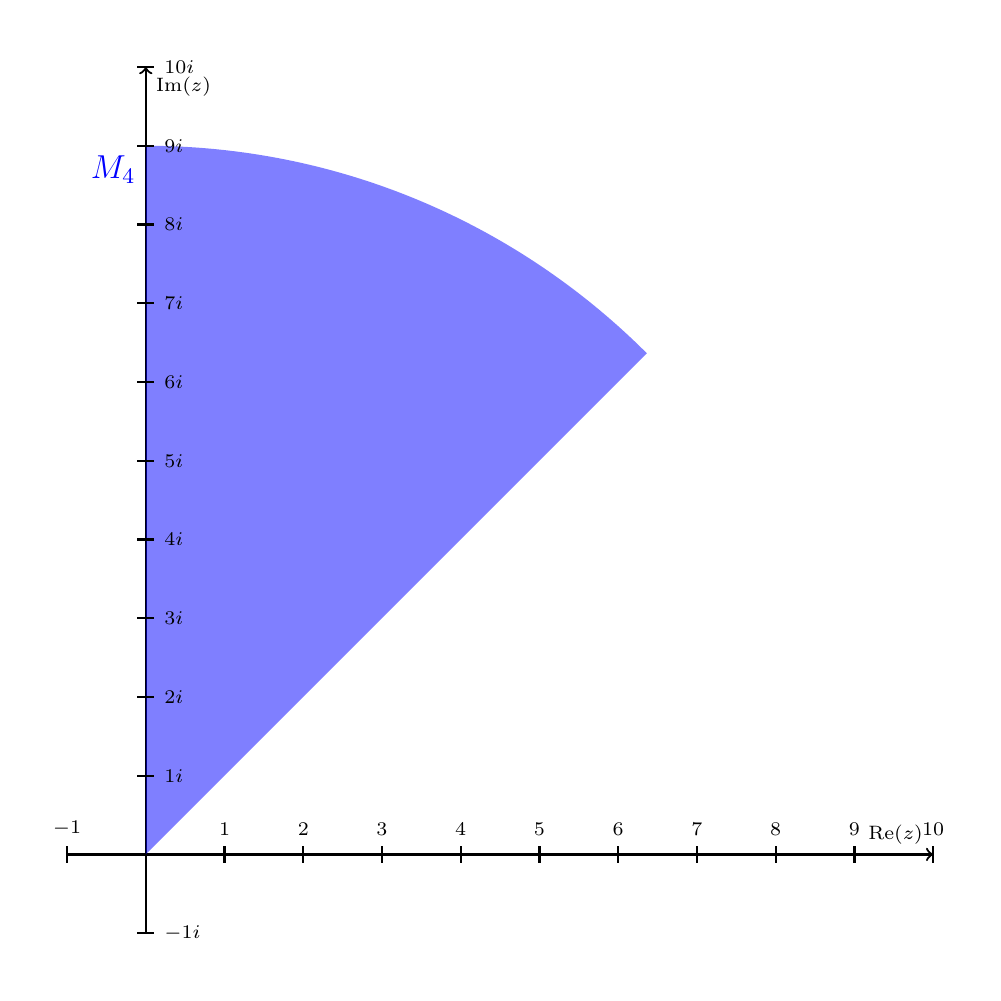
\begin{tikzpicture}
    \begin{scope}[thick,font=\scriptsize]
        \clip (-1.5,-1.5) rectangle (10.5,10.5);
        \draw [->] (-1,0) -- (10,0) node [above left]  {Re$(z)$};
        \draw [->] (0,-1) -- (0,10) node [below right] {Im$(z)$};
        \begin{scope}
            \clip (0,0) circle (9);
            \path [draw=none,fill=blue,opacity = 0.5] (0,0) -- (9,9) -- (0,9) node[pos=1, below left, color=blue, opacity=1] {\large$M_4$};
        \end{scope}

        \foreach \n in {-1,1,2,...,10}{%
            \draw (\n,-3pt) -- (\n,3pt)   node [above] {$\n$};
            \draw (-3pt,\n) -- (3pt,\n)   node [right] {$\n i$};
        }
    \end{scope}
\end{tikzpicture}
\end{document}
